\documentclass[a4paper,11pt]{article}
\usepackage[right=1in,left=1in,top=0.7in,bottom=0.7in]{geometry}
\usepackage{lipsum}
\usepackage{graphicx}
\usepackage{float}
\usepackage{cite}
\usepackage{color}
\usepackage{caption}
% \usepackage{listings}
% \usepackage{hyperref}
% \usepackage{textgreek}

\renewcommand{\familydefault}{\sfdefault}


\begin{document}
    \begin{titlepage}
        \begin{center}
            
\includegraphics[height=7.5em]{../resources/unilogo.png}
            \vspace{6em}

            {\LARGE Laboratory Protocol} \\ 
            {\huge\bfseries Characterization of Protein Stability,\\ Catalysis and Aggregation}
            \vspace{3em}
            
            {\large\bfseries Molecular Biology and Biochemistry of Life}\\
            Winter Semester 2023-24
            \vspace{12em}

            {\bfseries Authors} \\ 
            Masine Janet Tränkner\\
            Syed Alisamar Husain
            \vspace{5em}

            {\bfseries Supervisor} \\ Dr.\ Titus M. Franzmann
        \end{center}
        
    \end{titlepage}
    \pagebreak

    \tableofcontents
    \listoffigures
    \vspace{3em}
    {\noindent\Large\bfseries Author Information \vspace{0.75em}}\\
    \noindent\large Masine Janet Tränkner\\
    {\small MSc. Computational Modelling and Simulation}\\
    {\small Matriculation Number 5186813}\\
    {\it\small masine\_janet.traenkner@mailbox.tu-dresden.de}\\\vspace{0.5em}
    
    \noindent\large Syed Alisamar Husain\\
    {\small MSc. Computational Modelling and Simulation}\\
    {\small Matriculation Number 5198172}\\
    {\it\small syed\_alisamar.husain@mailbox.tu-dresden.de}
    \pagebreak

    \section{Temperature Induced Unfolding Transitions}
        The goal in this experiment is to determine the stability of the proteins Lysozyme and BSA 
        (Bovine Serum Albumin) at different concentrations, 2.5, 5 and 10 µM, by inducing unfolding 
        transitions through temperature changes.
        We detect unfolding using Fluorescence spectroscopy by measuring emission at 
        two wavelengths, 330nm and 350nm, and we expect to see a sharp increase in the ratio
        of these emissions when the protein unfolds.

        \subsection*{Measurements}
            The temperature was increased from 25 °C to 95 °C, at a rate of 2 °C per minute,
            and corresponding fluorescence at wavelengths 350nm and 330nm was measured.

            \begin{itemize}
                \item {\bfseries Lysozyme - Fluorescence vs. Temperature}
                \begin{figure}[H]
                    \centering
                    \begin{tabular}{cc}
                        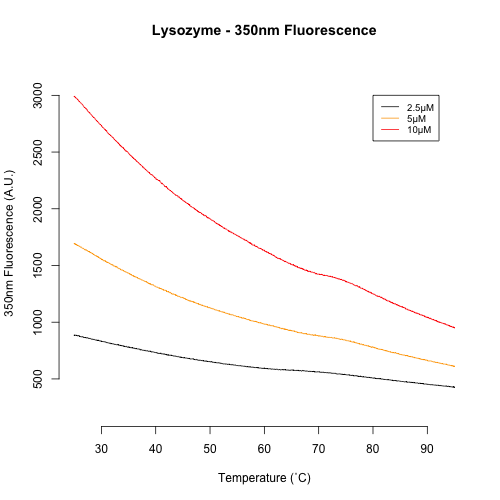
\includegraphics[width=180px]{../resources/unfolding_lys_350.png} &
                        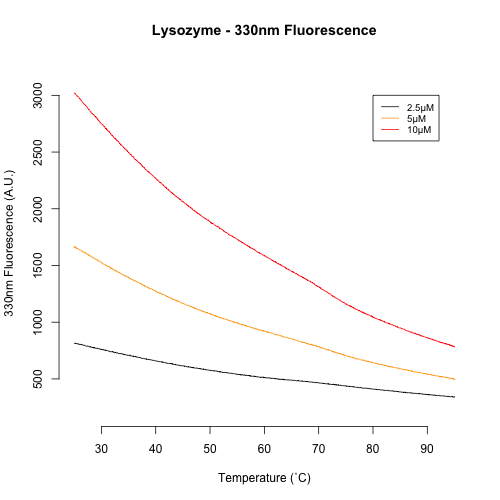
\includegraphics[width=180px]{../resources/unfolding_lys_330.png} \\
                        (a) & (b)\\
                    \end{tabular}
                    \caption{Lysozyme Fluorescence at wavelengths (a) 350nm and (b) 330nm}\label{fig:lys_flr}
                \end{figure}
                
                \item {\bfseries BSA - Fluorescence vs. Temperature}
                \begin{figure}[H]
                    \centering
                    \begin{tabular}{cc}
                        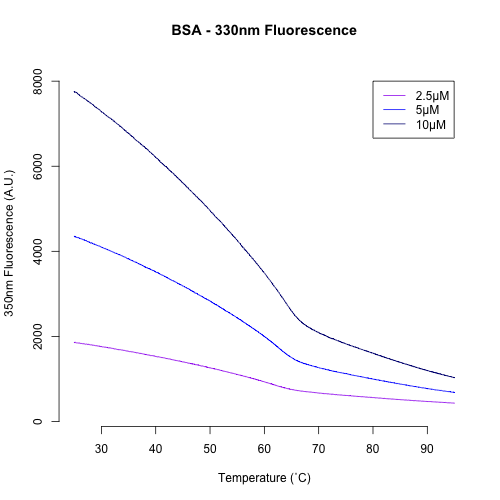
\includegraphics[width=180px]{../resources/unfolding_BSA_350.png} &
                        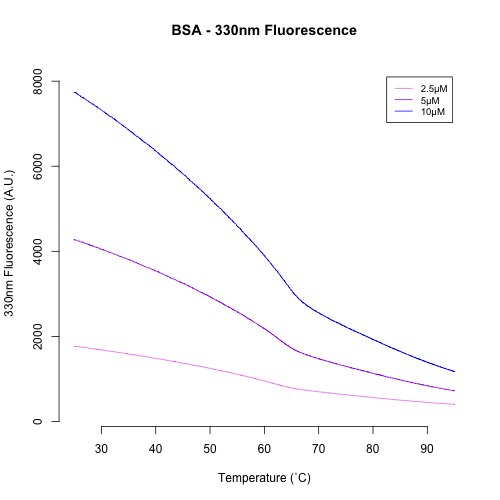
\includegraphics[width=180px]{../resources/unfolding_BSA_330.png} \\
                        (a) & (b)\\
                    \end{tabular}
                    \caption{BSA Fluorescence at wavelengths (a) 350nm and (b) 330nm}\label{fig:bsa_flr}
                \end{figure}
            \end{itemize}

        \subsection*{Analysis}
            The Fluorescence Ratio graph (Fig.~\ref{fig:temp_ratio}(a) and Fig.~\ref{fig:temp_ratio}(b)) was used to 
            approximate the transition midpoint. 
            Stability in the folded state arises from various interactions within the polypeptide. 
            However, upon surpassing a threshold temperature, the polypeptide 
            transitions to an unstable state. Consequently, as temperature increases, the population 
            of unfolded molecules also rises. This process behaves differently for the two proteins. 

            For Lysozyme, a low ratio can be observed at the beginning, which indicates that 
            the folded state predominates. With increasing temperature, this confirmation changes 
            up to a threshold temperature and the transition of the molecules into the unfolded state, 
            and accordingly the ratio also increases.
            \begin{figure}[H]
                \centering
                \begin{tabular}{cc}
                    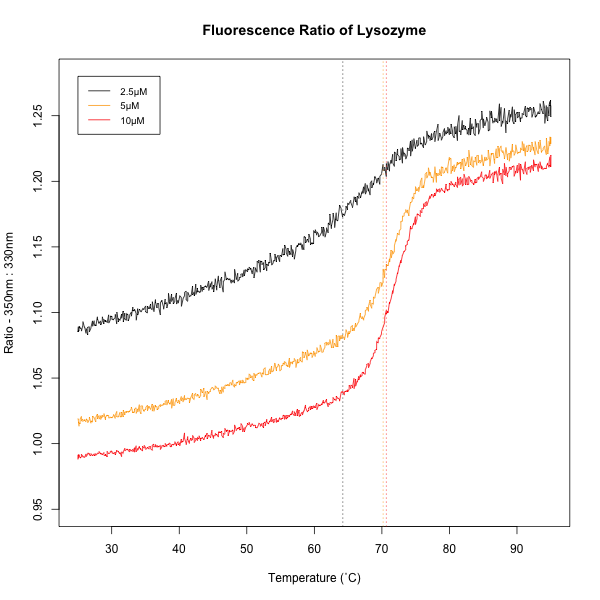
\includegraphics[width=200px]{../resources/unfolding_lys_ratio.png} &
                    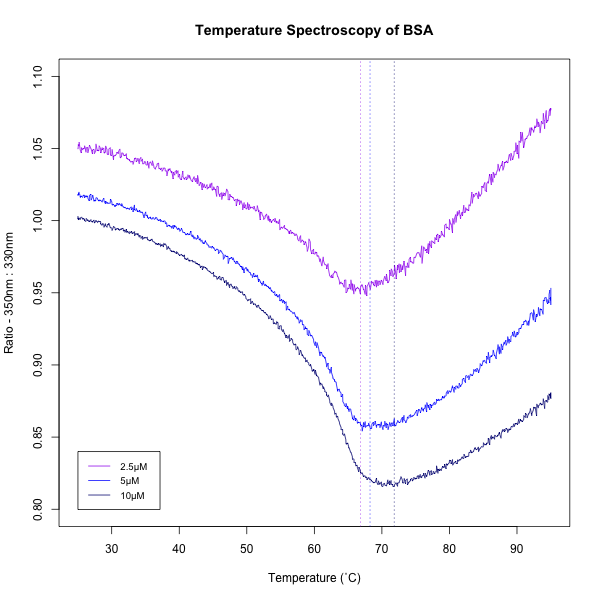
\includegraphics[width=200px]{../resources/unfolding_BSA_ratio.png} \\
                    (a) & (b)\\
                \end{tabular}
                \caption{Ratio of Fluorescence at 350nm to 330nm for (a) Lysozyme and (b) BSA}
                \label{fig:temp_ratio}
            \end{figure}
            
            The opposite can be observed for BSA. Here, the ratio is already high at the start of 
            the process and falls down to a certain threshold temperature. From this point, the ratio 
            increases for all concentrations and thus also the amount of proteins in the unfolded state.
            
            \begin{minipage}{0.5\textwidth}
                \begin{figure}[H]
                    \centering
                    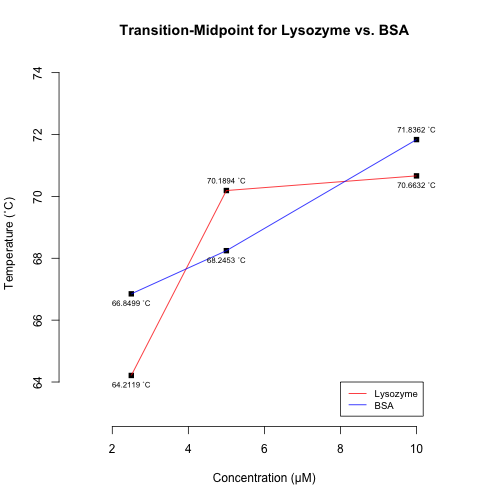
\includegraphics[width=\textwidth]{../resources/unfolding_tempVconc.png}
                    \caption{Ratio of Fluorescence at 350nm to 330nm for BSA}
                    \label{fig:temp_v_mid}
                \end{figure}
            \end{minipage}
            \begin{minipage}{0.45\textwidth}
                \vspace{-15em}
                The transition midpoints relative to concentration are plotted in Figure \ref{fig:temp_v_mid}.
                BSA shows a more linear temperature dependence than Lysozyme. 
            \end{minipage}
    \pagebreak
    
    \section{Lysozyme Aggregation Assay}
        In this experiment, aggregation of Lysozyme was studied to understand protein aggregation, 
        where unfolded polypeptide chains of the proteins Lysozyme and Hsp27 associate irreversibly, 
        leading to the formation of large particles that scatter light. 
        Throughout the experiment, Hsp27 was used to analyze its effect on the aggregation of 
        Lysozyme with presence of TCEP.
        
        \subsection*{Measurements}
            Detecting the actual scattering of light is a challenging task that requires more equipment.
            Instead, we measure absorbance as a proxy for scattering using a pulsed spectrometer.
            We choose a wavelength which we know is not absorbed by anything in the mixture and 
            we use that fact to say all of the intensity reduction is because of scattered light.
            \begin{figure}[H]
                \centering
                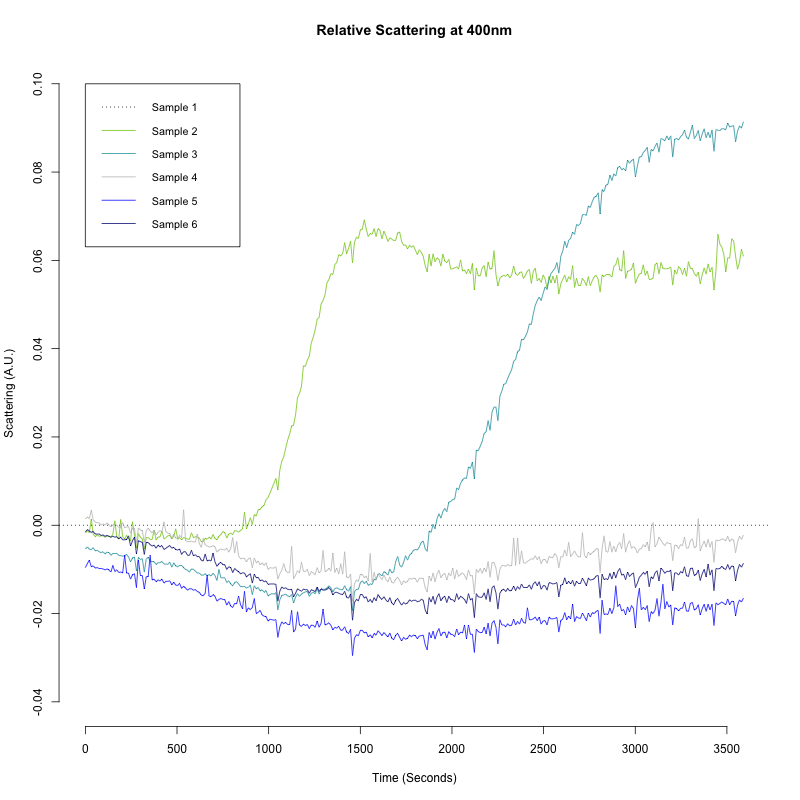
\includegraphics[width=350px]{../resources/aggregation_main.png}
                \caption{Scattering recorded as a function of time.}\label{fig:agg_main}
            \end{figure}

        \subsection*{Analysis}
            As protein aggregation increases, more light is scattered by the sample. 
            Introducing Hsp27 into the samples can regulate aggregation and consequently, 
            scattering. At low concentrations of Hsp27 (Samples 1 to 3 in Figure~\ref{fig:agg_main}), 
            Lysozyme aggregation isn't effectively inhibited. 
            Thus, the presence of Hsp27 in the solution increases overall absorption. 
            But it can also be seen that a higher concentration of 10 µM (Sample 3) delays the aggregation. 
            
            However, when the concentration of Hsp27 matches that of Lysozyme, aggregation is prevented, 
            resulting in lower absorbance (Sample 4). 
            The control samples lacking Lysozyme and denaturant exhibit no absorbance change at 400nm (Samples 5 and 6). 
            Only Samples 2 and 3 allow for the determination of an apparent halftime, which are $T^{S2}_{50\%} = 1200.30s$
            and $T^{S3}_{50\%} = 2422.34s$ respectively, as their curves display a change of conformation.
    \pagebreak
    
    \section{Michaelis-Menten Kinetics}
        Lactatdehydrogenase (LDH) catalyzes the reaction conversion of Pyruvate into Lactate. 
        In order to measure its activity the fluorescence of NADH, the cofactor of LDH, is measured 
        under 340nm light. As NADH is converted to NAD$^+$, this fluorescence reduces and reaches a 
        steady state when the reaction reaches equilibrium. We measure how fast this happens to determine
        the rate of reaction and find the Michaelis-Menten constants.
        
        \subsection*{Measurements}
            We measure the absorbance of 340nm light through a sample of the reaction mixture over time
            and plot this in Figure \ref{fig:mm_rates}. The slopes of these lines are directly proportional
            to the rates of reaction for each sample.
            \begin{figure}[H]
                \centering
                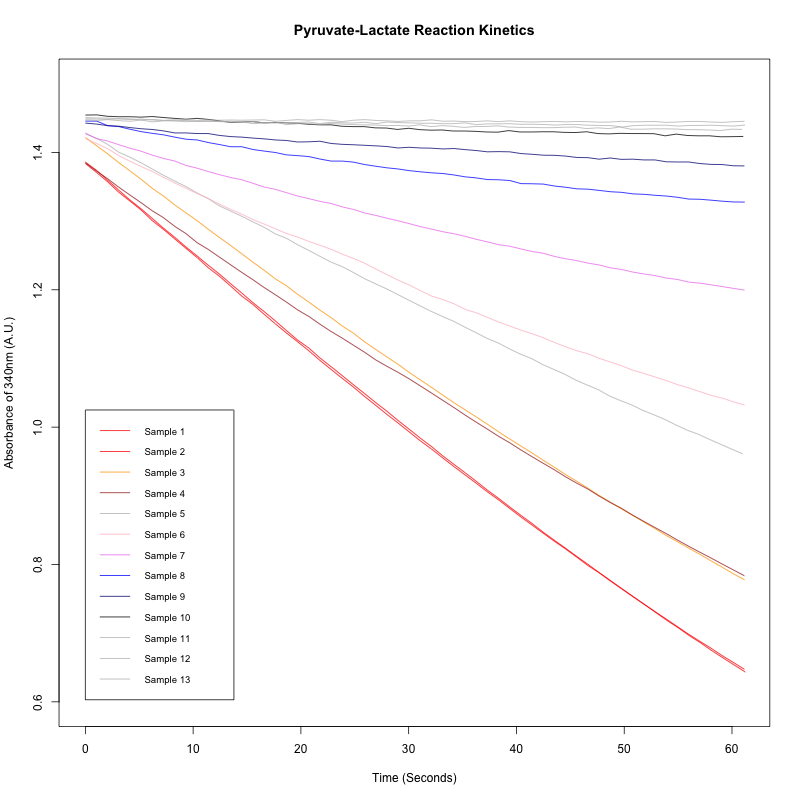
\includegraphics[width=350px]{../resources/kinetics_rates.png}
                \caption{Absorbance  as a function of time for different concentrations of Pyruvate}\label{fig:mm_rates}
            \end{figure}
            
            \subsection*{Analysis}
                The Michaelis-Menten plot (Fig.~\ref{fig:mm_plot}(a)) and the Lineweaver-Burk plot 
                (Fig.~\ref{fig:mm_plot}(b)) can be plotted from reaction rates derived 
                from change of absorbance over time, relative to the concentration of substrate. 
                It is evident that for low substrate concentrations, the rate of the reaction increases 
                linearly with increasing substrate concentration. As the substrate concentration increases, 
                the rate of the reaction eventually reaches a maximum value ($V_{max}$). 
                In this region, the active sites of the enzyme are largely occupied by the substrate, 
                and the rate becomes independent of further increases in substrate concentration.

                To find the maximum rate of reaction ($V_{max}$) and the Michaelis-Menten constant ($K_m$),
                we fit a linear model to the data, and the model estimates will give us an approximation of these constants.

                The Michaelis-Menten equation
                $ \frac{1}{V} = \frac{K_m}{V_{max}}\frac{1}{[S]} + \frac{1}{V_{max}} $
                is of the form
                $ y = \beta_1x + \beta_0 $.

                \begin{center}
                    Thus we have,
                    $ V_{max} = \frac{1}{\beta_0} $ and $ K_m = \frac{\beta_1}{\beta_0}  $
                \end{center}

                \begin{figure}[H]
                    \centering
                    \begin{tabular}{cc}
                        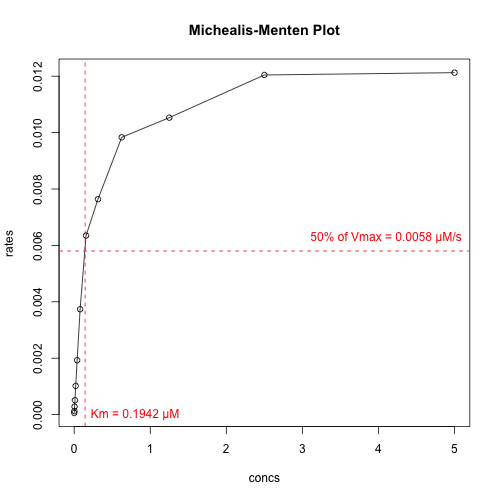
\includegraphics[width=220px]{../resources/kinetics_mmplot.png} &
                        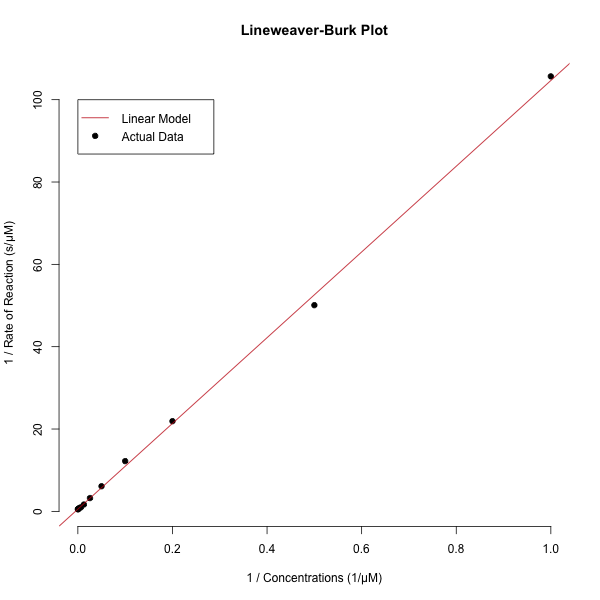
\includegraphics[width=220px]{../resources/kinetics_lbplot.png} \\
                        (a) & (b)\\
                    \end{tabular}
                    \caption{Michaelis-Menten plot and Lineweaver-Burk plot}\label{fig:mm_plot}
                \end{figure}

                \noindent From the linear model estimates we get $V_{max}$ = 1.8649 µM/s and for $K_m$ = 194.19 µM.\\
                We mark the value $V_{max}/2$ on the Michaelis-Menten plot (Fig.~\ref{fig:mm_plot}(a)), which can
                also give us the value of $K_m$ graphically. 
                In the Lineweaver-Burk plot (Fig.~\ref{fig:mm_plot}(b)) the slope of the fitted line indicates 
                the ratio $\frac{K_m}{V_{max}}$.\\

                To find the change in NADH concentration for each sample, we can use the absorbance formula
                of Lambert-Beer, $A = \epsilon d C$, we have,
                \begin{center}
                    $\Delta A = \epsilon d \Delta C$.
                \end{center}

                \begin{center}
                    Thus, $\Delta C = \frac{\Delta A}{\epsilon d}$,
                    where $\epsilon = 6220 M^{-1} cm^{-1}$ and $d = 1$ cm
                \end{center}
                
                Thus, change in NADH concentration is calculated from the change in absorbance.
                \begin{center}
                    \begin{tabular}{ c | c | c }
                        [Pyruvate] µM & $\Delta$A (A.U.) & $\Delta$[NADH] (µM) \\
                        \hline 
                        5000 & 0.7425 & 119.3729 \\
                        2500 & 0.7365 & 118.4083 \\
                        1250 & 0.6441 & 103.5530 \\
                         625 & 0.6013 & 96.67202 \\
                         313 & 0.4660 & 74.91961 \\
                         156 & 0.3884 & 62.44372 \\
                          78 & 0.2286 & 36.75241 \\
                          39 & 0.1179 & 18.95498 \\
                          20 & 0.0623 & 10.01607 \\
                          10 & 0.0311 & 4.999999 \\
                           5 & 0.0173 & 2.781350 \\
                           2 & 0.0076 & 1.221864 \\
                           1 & 0.0036 & 0.578778 \\
                    \end{tabular}
                \end{center}

    \pagebreak

    \section{UV/VIS Spectroscopy of NADH}
    Similar to the kinetics experiment, the concentration should also be measured here using UV/VIS spectroscopy.
    The detected absorbance should show local maxima for 3 specific wavelengths (208, 260 and 340 nm). It is also to be expected that the absorbance also increases with increasing NADH concentration. However, according to figure x, the absorbance increases from sample 1 to 3, then increases for the samples 4 and 5 and again increases for sample 6, without exceeding the highest absorbance of sample 2. 

        \begin{figure}[H]
            \centering
            \begin{tabular}{cc}
                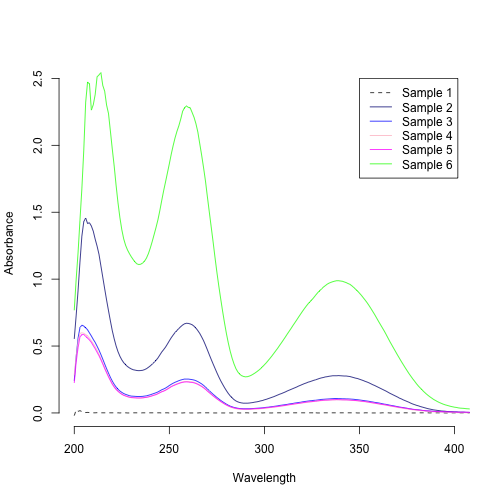
\includegraphics[width=200px]{../resources/absorption_r1_spectrum.png} &
                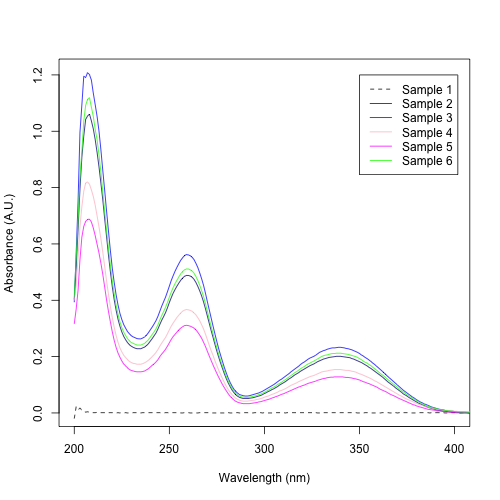
\includegraphics[width=200px]{../resources/absorption_r2_spectrum.png} \\
                (Run 1) & (Run 2)\\
            \end{tabular}
            \caption{Absorbance spectrum of NADH for different concentrations}
            \label{fig:abs_spectrum}
        \end{figure}

        \subsection*{Analysis}
            \begin{figure}[H]
                \centering
                \begin{tabular}{cc}
                    
\includegraphics[width=200px]{../resources/absorption_r1_340.png} &
                    
\includegraphics[width=200px]{../resources/absorption_r2_340.png} \\
                    (Run 1) & (Run 2)\\
                \end{tabular}
                \caption{Absorbance at 340nm for different concentrations}
                \label{fig:abs_340}
            \end{figure}
    \pagebreak

\end{document}